\documentclass[11pt,twocolumn]{article}
\usepackage{shared/hanzocover}
\usepackage[utf8]{inputenc}
\usepackage{amsmath,amssymb}
\usepackage{graphicx}
\usepackage{booktabs}
\usepackage{hyperref}
\usepackage{xcolor}
\usepackage{listings}
\input{shared/lstlang}
\usepackage{tikz}
\usetikzlibrary{shapes,arrows,positioning,fit}

\definecolor{codegreen}{rgb}{0,0.6,0}
\definecolor{codegray}{rgb}{0.5,0.5,0.5}
\definecolor{codepurple}{rgb}{0.58,0,0.82}
\definecolor{backcolour}{rgb}{0.95,0.95,0.92}

\lstdefinestyle{mystyle}{
    backgroundcolor=\color{backcolour},
    commentstyle=\color{codegreen},
    keywordstyle=\color{codepurple},
    numberstyle=\tiny\color{codegray},
    stringstyle=\color{codegreen},
    basicstyle=\ttfamily\footnotesize,
    breakatwhitespace=false,
    breaklines=true,
    captionpos=b,
    keepspaces=true,
    numbers=left,
    numbersep=5pt,
    showspaces=false,
    showstringspaces=false,
    showtabs=false,
    tabsize=2
}
\lstset{style=mystyle}

\title{Hanzo Insights: Privacy-First Product Analytics with Feature Flags and Real-Time Dashboards}
\author{Zach Kelling\thanks{zach@hanzo.ai} \\ \textit{Hanzo Industries} \\ \texttt{research@hanzo.ai}}
\date{April 2023}

\begin{document}

\hanzocoverpage

\begin{abstract}
We present Hanzo Insights, a privacy-first product analytics platform built on the Umami framework with ClickHouse as the analytical backend. Insights provides real-time event tracking, funnel analysis, cohort retention, and feature flag management without collecting personally identifiable information (PII). The system processes over 50 million events daily with sub-second query latency on dashboards spanning 90-day windows. Key innovations include: (1) a cookie-less visitor identification scheme using salted hashing of request attributes, (2) a feature flag engine with percentage rollouts, user targeting, and A/B experiment support, and (3) a streaming ingestion pipeline with at-most-once deduplication. Insights replaces Google Analytics and LaunchDarkly in the Hanzo stack, eliminating third-party data sharing while providing equivalent functionality.
\end{abstract}

\section{Introduction}

Product analytics platforms face a fundamental tension between data utility and user privacy. Traditional analytics services (Google Analytics, Mixpanel) rely on cookies and persistent identifiers to track users across sessions, creating privacy liabilities under GDPR, CCPA, and similar regulations. Privacy-focused alternatives (Plausible, Fathom) sacrifice granular event tracking and funnel analysis.

Hanzo Insights resolves this tension by combining Umami's~\cite{umami2020} cookie-less tracking approach with ClickHouse's~\cite{clickhouse2016} columnar storage for high-performance analytical queries. The result is a platform that provides detailed product analytics---funnels, cohorts, retention, custom events---without storing PII or requiring cookie consent banners.

\paragraph{Contributions.}
\begin{itemize}
    \item A cookie-less visitor identification scheme using daily-rotated salted hashes of IP address, User-Agent, and site identifier.
    \item A ClickHouse-backed analytical engine supporting sub-second queries over billions of events.
    \item An integrated feature flag system with percentage rollouts, targeting rules, and automatic experiment analysis.
    \item A real-time dashboard with live visitor counts, event streams, and configurable metric widgets.
\end{itemize}

\section{Architecture}

\subsection{System Design}

\begin{figure}[t]
\centering
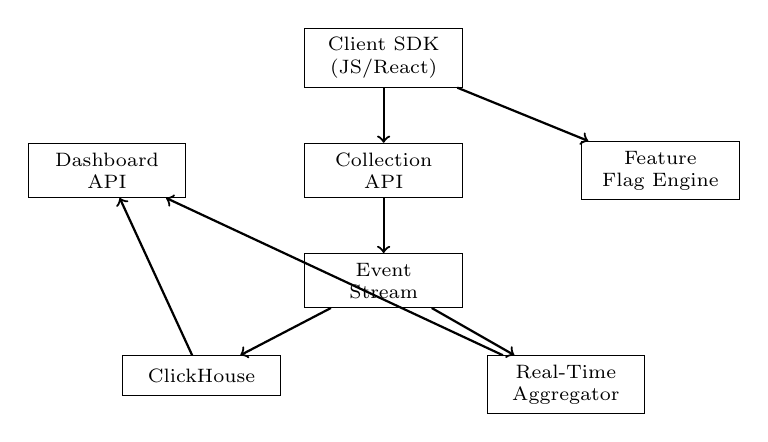
\begin{tikzpicture}[
    node distance=0.7cm,
    box/.style={rectangle, draw, minimum width=2cm, minimum height=0.5cm, align=center, font=\scriptsize},
    arrow/.style={->, thick}
]
\node[box] (sdk) {Client SDK\\(JS/React)};
\node[box, below=of sdk] (collect) {Collection\\API};
\node[box, below=of collect] (stream) {Event\\Stream};
\node[box, below left=0.6cm and 0.3cm of stream] (ch) {ClickHouse};
\node[box, below right=0.6cm and 0.3cm of stream] (rt) {Real-Time\\Aggregator};
\node[box, right=1.5cm of collect] (flags) {Feature\\Flag Engine};
\node[box, left=1.5cm of collect] (dash) {Dashboard\\API};

\draw[arrow] (sdk) -- (collect);
\draw[arrow] (collect) -- (stream);
\draw[arrow] (stream) -- (ch);
\draw[arrow] (stream) -- (rt);
\draw[arrow] (sdk) -- (flags);
\draw[arrow] (ch) -- (dash);
\draw[arrow] (rt) -- (dash);
\end{tikzpicture}
\caption{Insights data pipeline from collection to dashboard.}
\label{fig:insights}
\end{figure}

Events flow through a three-stage pipeline (Figure~\ref{fig:insights}): collection, streaming, and storage. The client SDK sends events to the Collection API, which validates, deduplicates, and forwards them to an event stream. ClickHouse consumes the stream for persistent storage, while the Real-Time Aggregator maintains in-memory counters for live dashboards.

\subsection{Visitor Identification}

Insights identifies visitors without cookies or persistent identifiers:

\begin{equation}
    \text{visitor\_id} = \text{SHA256}(\text{ip} \| \text{ua} \| \text{site\_id} \| \text{salt}_d)
\end{equation}

The daily salt $\text{salt}_d$ rotates at midnight UTC, ensuring that visitor identifiers cannot be correlated across days. This provides session-level analytics (pageviews, events within a visit) without cross-session tracking.

\subsection{Event Schema}

Events are stored in a ClickHouse MergeTree table:

\begin{lstlisting}[language=TypeScript]
interface Event {
  siteId: string;
  visitorId: string; // daily-rotated hash
  sessionId: string;
  timestamp: number;
  type: 'pageview' | 'event' | 'identify';
  url: string;
  referrer: string;
  name?: string;     // custom event name
  data?: Record<string, string>;
  country: string;   // from IP, not stored
  device: string;    // parsed from UA
  browser: string;
  os: string;
}
\end{lstlisting}

The table is partitioned by month and ordered by \texttt{(siteId, timestamp)}, enabling efficient range scans for dashboard queries.

\section{Key Features}

\subsection{Feature Flags}

The integrated feature flag engine evaluates flags server-side or client-side:

\begin{lstlisting}[language=TypeScript]
const flags = await insights.getFlags({
  userId: user.id,
  attributes: { plan: 'pro', country: 'US' }
});

if (flags['new-checkout']) {
  renderNewCheckout();
}
\end{lstlisting}

Flag rules support percentage rollouts (consistent hashing by user ID), attribute-based targeting, and mutual exclusion groups for A/B experiments. Flag evaluations are logged as events, enabling automatic analysis of flag impact on conversion metrics.

\subsection{Funnel Analysis}

Funnels are defined as ordered sequences of events:

\begin{lstlisting}[language=TypeScript]
const funnel = await insights.funnel({
  siteId: 'site_abc',
  steps: [
    { type: 'pageview', url: '/pricing' },
    { type: 'event', name: 'click_signup' },
    { type: 'pageview', url: '/onboarding' },
    { type: 'event', name: 'complete_setup' }
  ],
  window: '7d'
});
// Returns: [1000, 420, 310, 185]
\end{lstlisting}

ClickHouse's \texttt{windowFunnel} function evaluates multi-step funnels in a single query, avoiding the N+1 query pattern common in traditional analytics databases.

\subsection{Real-Time Dashboard}

The dashboard displays live metrics using Server-Sent Events (SSE). The Real-Time Aggregator maintains sliding window counters in memory, flushed to ClickHouse every 10 seconds. Dashboard widgets include: active visitors, pageviews per minute, top pages, referrer breakdown, geographic distribution, and device/browser splits.

\section{Implementation}

Insights is implemented as a Go service (18,000 lines) with a React dashboard (12,000 lines). The collection endpoint processes events in batches of 1,000, inserting into ClickHouse via the native protocol for maximum throughput.

\begin{table}[h]
\centering
\caption{Query latency on 90-day window (ms).}
\label{tab:query}
\begin{tabular}{lrr}
\toprule
\textbf{Query} & \textbf{p50} & \textbf{p99} \\
\midrule
Dashboard overview & 45 & 180 \\
Funnel (4 steps) & 120 & 450 \\
Cohort retention & 200 & 800 \\
Custom event count & 25 & 90 \\
Feature flag impact & 150 & 520 \\
\bottomrule
\end{tabular}
\end{table}

\section{Security}

\paragraph{No PII Storage.} IP addresses are used only for visitor hashing and geolocation, then discarded. User-Agent strings are parsed into device/browser/OS categories and discarded. The raw identifiers never reach ClickHouse.

\paragraph{Data Isolation.} Each tenant's data is scoped by \texttt{siteId}. ClickHouse queries include a mandatory \texttt{siteId} predicate enforced at the API layer. Cross-tenant queries are impossible by construction.

\paragraph{Collection Security.} The collection endpoint validates the origin header against registered site domains, preventing unauthorized event submission. Events exceeding 8KB are rejected.

\paragraph{GDPR Compliance.} Because Insights stores no PII, there is no personal data to delete, export, or consent to. The daily salt rotation ensures that visitor hashes are inherently time-limited.

\section{Conclusion}

Hanzo Insights demonstrates that privacy-first analytics need not sacrifice functionality. By combining cookie-less visitor identification with ClickHouse's columnar storage, Insights provides funnel analysis, cohort retention, and feature flag management with sub-second query latency---all without storing personally identifiable information. The integrated feature flag engine eliminates the need for a separate service, reducing infrastructure complexity while enabling data-driven product decisions.

\bibliographystyle{plain}
\begin{thebibliography}{10}

\bibitem{umami2020}
M. Cao. Umami: Simple, fast, privacy-focused website analytics. 2020.

\bibitem{clickhouse2016}
ClickHouse Inc. ClickHouse: Open-source column-oriented database management system. 2016.

\bibitem{gdpr2016}
European Parliament. General Data Protection Regulation (GDPR). 2016.

\bibitem{plausible2019}
Plausible Analytics. Plausible: Simple and privacy-friendly Google Analytics alternative. 2019.

\end{thebibliography}

\end{document}
